
La premi�re partie est de consuitre les topologies virtualis�es et de
tester les performances de MTPCP en faisant varier les param�tres des
sous-flots. La seconde partie est de construire un alogrithme
d'ordonnancement r�pondant � des crit�res de s�curit�.
\vspace{0.5cm}

Les �tapes du d�veloppement suivront les points suivants:

\begin{itemize}
\item Pr�paration d'une machine mininet avec le noyau MPTCP compil�
  pour l'ensemble de l'�quipe:
\item Lecture, compr�hension et commentaires du code de MPTCP;
\item Pr�paration de plusieurs topologies : \emph{fat tree} pour
  simuler un \emph{data center} et une topologie permettant de tester
  la concurrence entre MPTCP et TCP;
\item Pr�paration d'une biblioth�que de tests et de mesures via l'API python;
\item \'Ecriture d'un algorithme d'ordonnancement dans le noyau;
\item Mesures de performance.
\end{itemize}



\subsection{Descriptif du travail de Quentin Dubois et de Kevin Lam}
\begin{figure}[!htb]
  \begin{changemargin}{-2.0cm}{0.5cm}
    \centering
    \includegraphics[width=1.2\textwidth]{../gantt/KevinQuentin.png}
  \end{changemargin}
  \centering
  
  \caption{\textbf{Diagramme de Gantt Kevin Lam et Quentin Dubois}. }
  \label{fig:gantt}
\end{figure}

Analyse de la structure de l'impl�mentation :
	\begin{itemize}
		\item D�terminer globalement les fichiers � lire ;
		\item D�finir les headers et structures li�s � l'utilisation de mptcp.
	\end{itemize}\\

Lecture et Compr�hension du code :
	\begin{itemize}
   		\item Lecture de tous les fichiers contenus dans \$(SRC\_NOYAU)/net/mptcp ;
   		\item Lecture de certains fichiers contenus dans \$(SRC\_NOYAU)/net/sched ;
	   \item Lecture de tous les types/structures utilis�s ;
	   \item Relecture du code apr�s avoir compris tous le types/structures.
	\end{itemize}\\

D�finition des parties modifiables de l'ordonnanceur :
	\begin{itemize}
	   \item V�rifier les correspondances entre mptcp\_output.c et mptcp\_input.c ;
	   \item Voir si l'utilisation du contr�le de congestion (mptcp\_olia.c et mptcp\_coupled.c) a des effets de bord sur les sockets ;
	   \item Voir les diff�rences entre les diff�rents modes du path\_manager.
	\end{itemize}\\

Impl�mentation / Tests d'algorithmes pour l'ordonnanceur :
	\begin{itemize}
		\item Avec l'aide de Matthieu Coudron, modification dans
		\$(SRC\_NOYAU)/net/mptcp/mptcp\_output.c ;
	   \item Tests des impl�mentations avec le travail de Romain LY et comparer les r�sultats obtenus.
   	\end{itemize}\\


\subsection{Descriptif du travail de Romain Ly}
\begin{figure}[!htb]
  \begin{changemargin}{-2.0cm}{0.5cm}
    \centering
    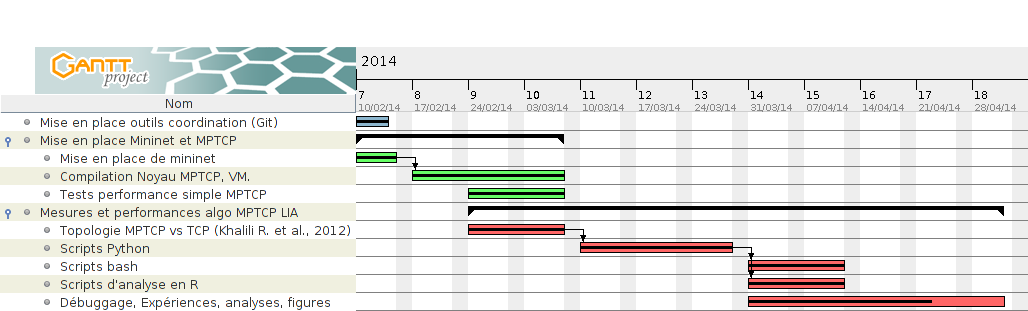
\includegraphics[width=1.2\textwidth]{../gantt/romain.png}
  \end{changemargin}
  \centering
  
  \caption{\textbf{Diagramme de Gantt de Romain Ly.}}
  \label{fig:gantt}
  
\end{figure}

\begin{itemize}
\item Mise en place du Git
\item Compilation noyau MPTCP dans la VM mininet et tests simples de routines
\item Topologie modifi�e de Khalili et al.
\item Scripts Python
  \begin{itemize}
  \item impl�mentation d'un parseur d'arguments
  \item int�gration de ping, iperf, iperf3, bwm-ng, sshd, tcpdump
    permettant le monitoring et l'�tude du r�seau
  \end{itemize}
\item Installation de TCP-reduce dans la VM pour v�rifier les options de la connexion TCP.
\item Scripts Bash pour g�n�rer de multiples simulations par l'interm�diaire de scripts Python
\item Scripts R pour analyse des r�sultats et figures
\item D�bogages des scripts
\item Exp�rimentations
  \begin{itemize}
  \item variation du nombre de sous flots, d�bits, latences, taille de
    fen�tre, etc.
  \end{itemize}
\end{itemize}


\subsection{Descriptif du travail de Simon Ravier}

\begin{figure}[!htb]
  \begin{changemargin}{-2.0cm}{0.5cm}
    \centering
    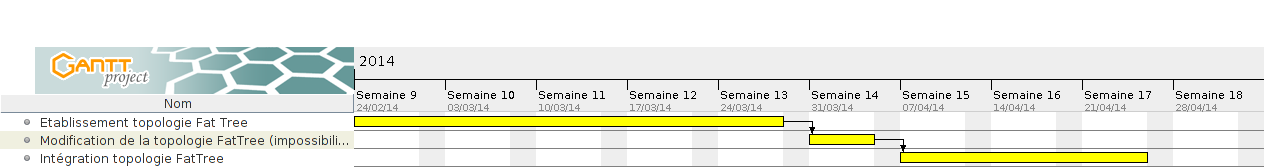
\includegraphics[width=1.2\textwidth]{../gantt/Simon.png}
  \end{changemargin}
  \centering
  
  \caption{\textbf{Diagramme de Gantt de Simon Ravier.}}
  \label{fig:gantt}
\end{figure}

\vspace{1cm}
\begin{tabular}{lp{12cm}}
  03/03 au 30/03 & �tablissement de la topologie FatTree\\
  31/03 au 06/04 & modification de la topologie FatTree (impossibilit� technique de r�aliser le premier mod�le)\\
  07/04 au 27/04 & Int�gration de la topologie FatTree dans
l'environnement de tests (configuration des h�tes, �tablissement des
tables de routage) et r�alisation des tests
\end{tabular}
\vspace{0.5cm}